\documentclass[12pt]{article}
%Gumm{\color{blue}i}|065|=)
\usepackage{amsmath, amsfonts, amssymb}
\usepackage[margin=0.5in]{geometry}
\usepackage{xcolor}
\usepackage{graphicx}

% zeta funct{\color{blue}i}ons of cub{\color{blue}i}c f{\color{blue}i}elds

%\usepackage{p{\color{blue}i}font}
\usepackage{amsmath}

\newcommand{\off}[1]{}
\DeclareMathSizes{20}{30}{20}{18}

\newcommand{\two }{\sqrt[3]{2}}
\newcommand{\four}{\sqrt[3]{4}}





\usepackage{tikz}

\newcommand{\susy}{{\bf Q}}
\newcommand{\RV}{{\text{R}_\text{V}}}

\title{Scratchwork: Torus Orbits}
\date{}
\begin{document}

%\fontfam{\color{blue}i}ly{qag}\selectfont \fonts{\color{blue}i}ze{12.5}{15}\selectfont

\sffamily

\maketitle

\noindent A common step in contemprary number theory literature is to re-define the problem as a group theory problem\dots Especially using ``torus orbits".  \\ \\
Linear algebra works over any field, $K$.  So we just say ``let $K$ be a field\dots" and if we have a single plane $\mathbb{R}^m \subseteq \mathbb{R}^n$ we know more-or-less they all behave the same.  In fact, rational planes $\mathbb{Q}^m \subseteq \mathbb{Q}^n$ are not all identical.
$$ X(\mathbb{Q}) = \{ x^2 + y^2 = 1 \}  \subseteq \mathbb{Q}^2 $$
This is a $\mathbb{Q}$-torus.  Are there any rational points on this circle?  I can name $(0,\pm1)$ and $(\pm 1,0)$.  Here are two more:
$$ (\tfrac{3}{5}, \tfrac{4}{5}) , (\tfrac{5}{13}, \tfrac{12}{13}) \in X(\mathbb{Q}) $$
Since the circle was defined using algebra, we can say it is a \textbf{variety}.  In fact, $X(\mathbb{Q})$ forms a group:
$$ \left(\frac{3}{5} + i \, \frac{4}{5}\right)^2 
=  \left(\frac{3^2 - 4^2 }{25}\right) + 2 \times\left( \frac{3 \times 4}{25} \right)i =  - \frac{7}{25} + i \, \frac{24}{25}$$
Or we culd use $2 \times 2$ matrices.  There's a way find a $2 \times 2$ matrix solution to $x^2 + 1 = 0$. E.g. $(x,y) \mapsto (-y,x)$.
$$ \left[ 
\begin{array}{rr} \frac{3}{5} & -\frac{4}{5} \\  \\
\frac{4}{5} & \frac{3}{5} 
\end{array}
\right]^2 = \left[ 
\begin{array}{rr} \frac{7}{25} & -\frac{24}{25} \\ \\
\frac{24}{25} & \frac{7}{25} 
\end{array}
\right]$$
This tell us the Pythagorean triples form a \textit{multiplicative group}, but also we are looking for a $\mathbb{Q}$-action, and possibly an $\text{SL}_2(\mathbb{Z})$ action (I read it's actually a $\Gamma(2)$ action.)\\
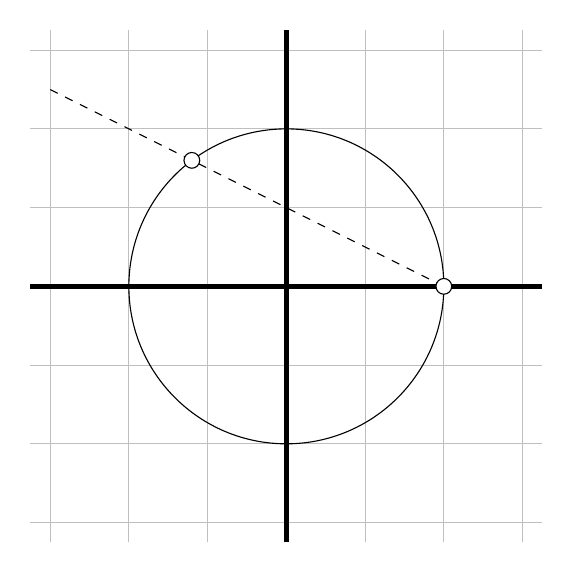
\begin{tikzpicture}
\foreach \a in {-3,...,3}{
	\draw[color=black!25!white] (\a,-3.25)--(\a,3.25);
	\draw[color=black!25!white] (-3.25,\a)--(3.25,\a);
}
\draw[color=black, line width=2] (-3.25,0)--(3.25,0);
\draw[color=black, line width=2] (0,-3.25)--(0,3.25);
\draw (0,0) circle (2);
\draw[dashed] (2,0)--(-3,2.5);
\draw[fill=white] ( 2,0) circle (0.1);
\draw[fill=white] (-1.2,1.6) circle (0.1);
\end{tikzpicture} \\
Notice we've used a tiny bit of degree theory $[circle]\cdot[line]=2 $.  This \textbf{is} an instance of cohomology\footnote{intersection theory} and we don't bother giving it a fancy name.  This is called \textbf{stereographic projection}, I think? 
\begin{eqnarray*}\big|(1,0)+ (t, mt) \big|^2 = (t+1)^2 + mt^2 &=& 1 \\
t  &=& (1,0) ,   (\tfrac{1-m^2}{m^2 + 1},- \tfrac{2m}{m^2+1}) \end{eqnarray*}
with $m = \frac{a}{b} \in \mathbb{Q}$.  These become $[a^2 - b^2 :2ab: a^2 + b^2]$ over $\mathbb{Z}$ as a proportion.  Multiplying by the slope $m \mapsto q x$ could lead to a reasonable group action of $\mathbb{Q}^\times$ on $\mathbb{Q}$. \\ \\
\textbf{Ex} Show no such $\mathbb{Q}^\times$ action exists on $\text{SO}_2(x^2 + y^2, \mathbb{Q})$.   \\ \\
In fact, showing that \textit{no} isomorphism (or group) action exists might be quite hard.  Now I just want to soak in that $\text{SO}_2$ for various quadratic forms are now quite different.  This is how we can talk about \textbf{rational quadratic forms}.
\begin{eqnarray*}
\text{SO}_2(x^2 + y^2, \mathbb{Q}) &\not \simeq& \text{SO}_2(x^2 + 2y^2, \mathbb{Q}) 
\not \simeq \text{SO}_2(x^2 -2 y^2, \mathbb{Q})  \\ 
\text{SO}_2(x^2 + y^2, \mathbb{R}) & \simeq& \text{SO}_2(x^2 + 2y^2, \mathbb{R}) 
 \not\simeq \text{SO}_2(x^2 -2 y^2, \mathbb{R})\end{eqnarray*}  
since we do have $\sqrt{2} \in \mathbb{R}$, but not $\sqrt{-2} \in \mathbb{R}$. So letting the quadrtaic form $q \in M_{2 \times 2} (\mathbb{Q})$ vary we can obtaion lots of different infinite abelian groups, roughly the size of $\mathbb{Q}^\times$.  These are call $\mathbb{Q}$-tori and if there was such an isomorphism -- the matrices could be diagonalized over $\mathbb{Q}$ -- then these would be called \textbf{split torus}. \\ \\
Here is another torus build to the same variety $X = \{ x^2 + y^2 - 1 = 0\}$ a circle.  Let's consider $X\big(\mathbb{Q}(\sqrt{2})\big)$.  The points on the circle living in the field $\mathbb{Q}[x]/(x^2 - 2)$.  Since $\sqrt{2} \notin \mathbb{Q}$ this is a slightly bigger field and we have ``more" points.  Nonetheless 
$$ \overline{\mathbb{Q}} = \overline{\mathbb{Q}(\sqrt{2})} = \mathbb{R}  \to X(\mathbb{Q}) \subseteq X(\mathbb{Q}(\sqrt{2})) \subseteq X(\mathbb{R})   
\to \overline{X(\mathbb{Q})} = \overline{X(\mathbb{Q}(\sqrt{2}))} = X(\mathbb{R})   $$
What allows us to make that conclusion so easily?  The closure operation $\overline{(\cdot)}$ comes from \textbf{topology} -- basically a way of deciding which sets of points are ``close" or ``nearby" or ``related" or ``approximate".
\begin{eqnarray*} (a_1 + a_2 \sqrt{2})^2 + (b_1 + b_2 \sqrt{2})^2 &=& (c_1 + c_2 \sqrt{2})^2 \\ 
(a_1^2 + 2a_2^2 ) + (b_1^2 + 2b_2^2 ) &=& (c_1^2 + 2c_2^2 )  \\ 
a_1 a_2 + b_1 b_2 = c_1c_2\end{eqnarray*}
And usually there's some trick that I'm overlooking.  Hopefully we can find a readin of these equations from within Euclidean Geometry, where this equation originated.\\ \\
\textbf{Ex} Let's try solving $x^2 + y^2 + z^2 = n$ as a torus orbit of some kind.  This exercise is worked out in a handful of places.\footnote{My standard for well-known is that everybody knows it.  There are only 20000 practicing mathematicians in the US, maybe a tenth of those are number theorists.  So... } I'm going to ask for the automorphic representation $\pi$ of $\text{SL}_2(\mathbb{A})$ for a spherical harmonic $\phi \in L^2( \text{SO}_3)$. \\ \\
How do theta-functions occur as automorphic representations?  This is possibly called the ``Weil representation" or the ``Metaplectic" representation.\footnote{However, when talking to professors (or reading their work) there's steep cliff separating the people who know the Automorphic Forms jargon and the people who do not.  And even another cliff between factions of professions (e.g. Automoprhic Forms and Number Theory).  This is a socical network analysis (SNA) phenomenon\dots}  I'll concede that Waldspurger formula has been known since 1980, but his derivtion takes about 30 or 40 pages and he never ``evaluates" the thing.  It's on me, to define this term \textbf{evaluate}. \\ \\
Conversely, since equidstirbution statements (i.e. uniform distribution of points on $S^2$) is so hard, we can find statements about the uniform distribution and say that our solutions $X(\mathbb{Z},n)$ are ``close to" being examples of inputs.  There could be a whole theory of not-quite-uniform points on the 2-sphere \\ \\
Paul Nelson works through this in 2016, and it look like Waldspurger's computations - and \textit{he} says these calculations are new.  So change is pretty slow.

\newpage

\noindent \textbf{Ex} Find a sequence of rational numbers $x_n \in \mathbb{Q}$ converging to $\sqrt{2} \in \mathbb{R}$ and $\sqrt{-1} \in \mathbb{Q}_5$.
$$ \big| \big(\tfrac{p}{q}\big)^2 -2 \big|_\mathbb{R} < \epsilon_1 \text{ and }
\big|\big(\tfrac{p}{q}\big)^2 + 1 \big|_{5} < \epsilon_2 $$
Let's make sure the second one exists.  $2^2 + 1 = 5 \in 5 \mathbb{Z}$ and $3^2 + 1 = 2 \times 5 \in 5 \mathbb{Z}$.  This tell us there should be two numbers $x_\pm = \sqrt{-1} \in \mathbb{Q}_5$ by Hensel's Lemma (basically Taylor formula).
$$ \text{diag} : \tfrac{p}{q} \in \mathbb{Q} \to 
(\tfrac{p}{q} , \tfrac{p}{q} ) \in \mathbb{Q} \times \mathbb{Q} \to \mathbb{R} \times \mathbb{Q}_5 $$
I don't have a great notation for it. $\overline{\text{diag}(\mathbb{Q} \times \mathbb{Q})} = \mathbb{R} \times \mathbb{Q}_5$.  The algebra is telling us by attemping to \textit{define} the word ``diagonal" or the density of $\mathbb{Q}$ in such a big space as $\mathbb{R} \times \mathbb{Q}_5$ we've missed something even bigger. \\ \\
\textbf{Ex} Let's try to quantify how dense the rational points are on the circle? Let's find a $k \in \mathbb{Z}$ such that: 
$$  \min_{(p,q) \in \mathbb{Z}} \Big|( \tfrac{1}{\sqrt{2}} - \tfrac{p}{q})^2 + (\tfrac{1}{\sqrt{2}} - \tfrac{p}{q})^2 \Big|  \asymp q^k $$
Just a thought.

\vfill

\begin{thebibliography}{}

\item David Witte Morris \textbf{Introduction to Arithmetic Groups} \texttt{arXiv:math/0106063}

\item John Voight \textbf{Quaternion Algebras \texttt{(v.0.9.13)}} \texttt{https://math.dartmouth.edu/\~{}jvoight/quat.html}

\item Jean-Loupe Waldspurger \textbf{Sur les Valeurs de Certaines Fonctions L Automorphes en leur Centre de Sym\'{e}trie} Compositio Mathematica 54.2 (1985): 173-242. \texttt{<http://eudml.org/doc/89702>}.

\item Paul D Nelson \textbf{The spectral decomposition of $|\theta|^2$} \texttt{arXiv:1601.02529}

\end{thebibliography}
\end{document}